
%%%%%%%%%%%%%%%%%%%%%%%%%%%%%%%%%%%%%%%%%%%%%%%%%%%
%% Capítulo 1: El Concepto de Fractal
%%%%%%%%%%%%%%%%%%%%%%%%%%%%%%%%%%%%%%%%%%%%%%%%%%%


Las primeras preguntas que se pueden plantear son ¿qué es un fractal? ¿Qué tienen de especial estas figuras? ¿Qué las diferencia de un objeto no fractal? ¿Por qué es necesaria una geometría fractal? Trataremos de responder a cada una de estas preguntas a lo largo de este capítulo, comenzando por la primera de ellas. En realidad, hay distintas definiciones de \textit{fractal}, pero todas utilizan dos conceptos como base: la \textbf{autosimilaridad} y la \textbf{dimensión}. La primera de ellas es más cercana para nosotros de lo que en un principio podemos pensar, fijémonos en los ejemplos de la imagen \ref{fig:objetos}. 

\begin{figure}[h]
\begin{tabular}{cc}
  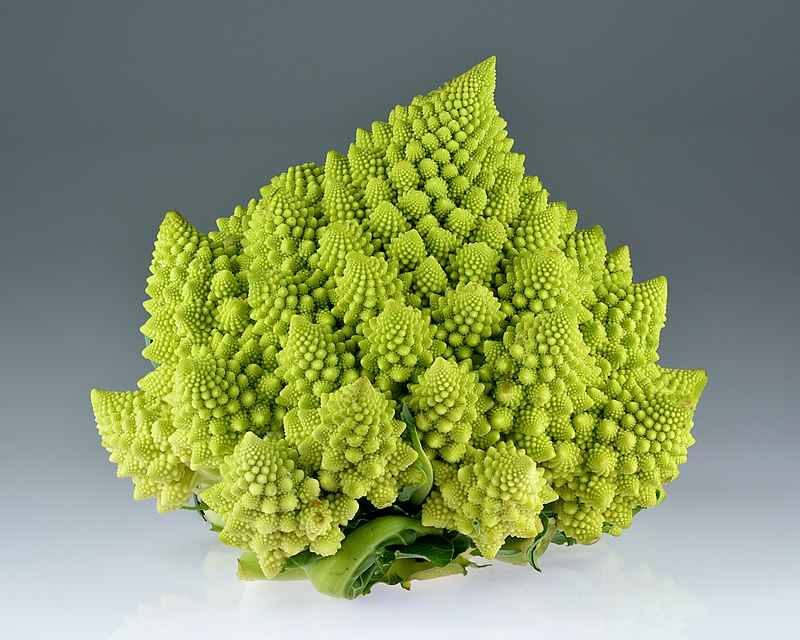
\includegraphics[scale=0.24]{./img/romanescu.jpg} &   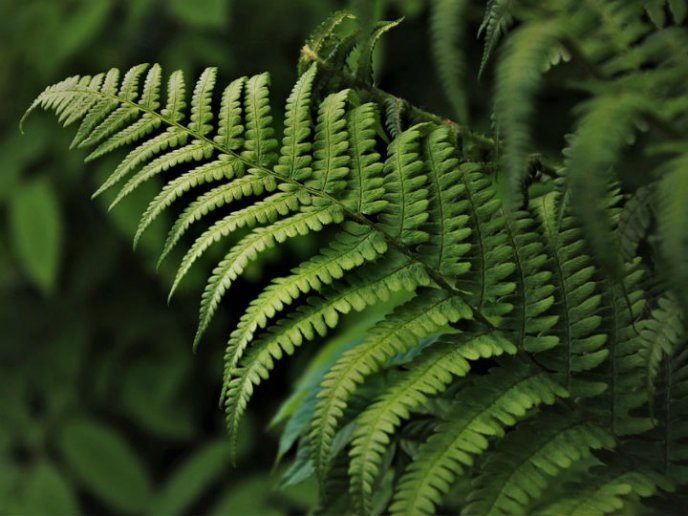
\includegraphics[scale=0.28]{./img/helecho.jpg} \\
(a) Romanescu & (b) Hoja de un helecho \\[6pt]
\end{tabular}
\caption{Objetos cotidianos con estructura fractal}
\label{fig:objetos}
\end{figure}

Observemos que el romanescu, que es un tipo de coliflor, pareciera que está formado de pequeños trozos que recuerdan el objeto original, mientras que estos pequeños trozos a su vez también están formados de pequeños trozos que recuerdan al original, y así sucesivamente. Por su parte, la hoja de un helecho también pareciera estar formada por muchas hojas más pequeñas similares a la original, y estas pequeñas hojas a su vez también están formadas por otras hojas aún más pequeñas.

Esta idea de objetos prácticamente iguales al original salvo cambios de escala es la subyacente al concepto de autosimilaridad.

\begin{definicion}[Autosimilaridad] Un objeto es \textbf{autosimilar} si está compuesto por copias de sí mismo reducidas mediante un factor de escala.
\end{definicion}

Para afianzar y formalizar conceptos y con el objetivo de introducir un concepto de dimensión, estudiaremos algunos ejemplos clásicos de objetos fractales.

\section{Ejemplos clásicos}
\label{section:ejemplos}

\subsection{El conjunto de Cantor}
\label{subsection:Cantor}

Creado por el célebre matemático \textit{George Cantor}, este fractal se construye a partir de un segmento de línea recta aplicando el siguiente proceso iterativo:

\begin{enumerate}
\item Dado el segmento de recta compuesto por el intervalo cerrado $[0,1]$, dividimos dicho segmento en tres segmentos iguales y extraemos el intervalo central, manteniendo los extremos. Es decir, extraemos el intervalo abierto $\left(\frac 1 3, \frac 2 3\right)$ y mantenemos el segmento $\left[0,\frac 1 3\right]$ y el $\left[\frac 2 3, 1\right]$. Nótese que obtenemos $2=2^0$ segmentos, cada uno a escala $\frac 1 3=\left(\frac 1 3\right)^1$ del original.

\item Aplicamos el mismo proceso a los segmentos $\left[0,\frac 1 3\right]$ y $\left[\frac 2 3, 1\right]$. Esto es, se dividen ambos en tres partes iguales y se extrae el intervalo abierto central de cada uno de ellos, manteniendo los extremos. En este caso obtendríamos $4=2^2$ segmentos iguales, cada uno de ellos a escala $\frac 1 3$ de los dos obtenidos en el primer paso y a escala $\frac 1 9=\left(\frac 1 3\right)^2$ del original.

\item Repetimos este proceso de manera indefinida, de manera que en el $n$-ésimo paso se obtendrían $2^n$ segmentos de recta a escala $\left(\frac 1 3\right)^n$.
\end{enumerate} 

Los puntos del intervalo inicial $[0,1]$ que restan tras las infinitas iteraciones son los que conforman el \textit{conjunto de Cantor}, que denotamos con $\textbf{C}$.

\begin{figure} [h]
\centering
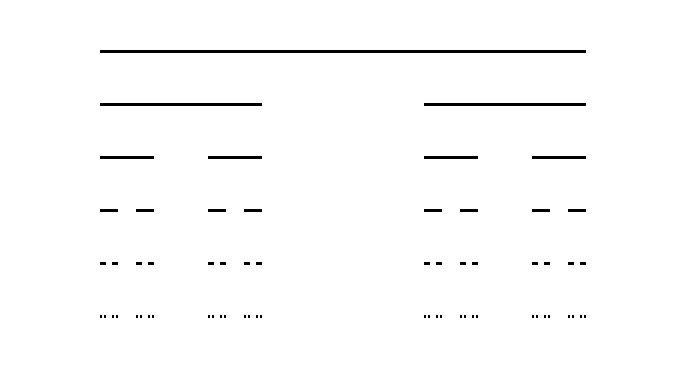
\includegraphics[scale = 0.5]{img/cantor.png}
\caption{Iteraciones del proceso de generación del conjunto de Cantor}
 \label{fig:Cantor}
\end{figure}

\subsection{La curva de Koch}
\label{subsection:curva-Koch}

Esta figura, creada por el sueco N. F. Helge von Koch sigue un proceso de construcción iterativo al igual que el conjunto de Cantor, pero en lugar de eliminar segmentos, se añaden de la siguiente manera (ver imagen \ref{fig:curva-Koch})

\begin{enumerate}
\item Partiendo de un segmento de recta de longitud $1$ (la longitud inicial es irrelevante, pues la figura final es la misma salvo un factor de escala), se divide en tres partes iguales de longitud $\frac 1 3$ y la parte central se sustituye por un triángulo equilátero al que se le elimina la base. Esto da lugar a $4=4^1$ segmentos de recta de longitud $\frac 1 3=\left(\frac 1 3\right)^1$.

\item Repetimos este proceso en cada uno de los segmentos de recta obtenidos, colocando el triángulo siempre por encima de la recta, obteniendo así $16=4^2$ segmentos de recta de longitud $\frac 1 9=\left(\frac 1 3\right)^2$.

\item Aplicamos este proceso indefinidamente, obteniendo en el paso $n$-ésimo $4^n$ segmentos de longitud $\left(\frac 1 3\right)^n$. 
\end{enumerate}

El resultado final del proceso es lo que llamamos la \textit{curva de Koch}, que denotamos como \textbf{K}.

\begin{figure} [h]
\centering
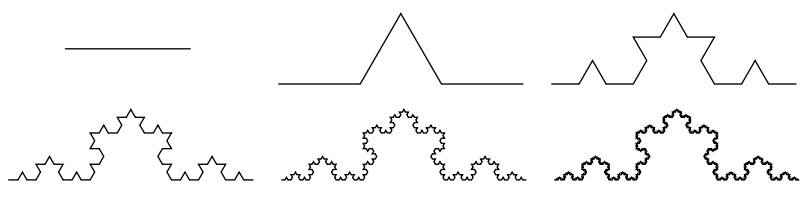
\includegraphics[scale = 0.6]{img/curva-Koch.png}
\caption{Iteraciones del proceso de generación de la curva de Koch}
 \label{fig:curva-Koch}
\end{figure}

\subsection{El copo de nieve de Koch}

A partir de la curva de Koch podemos crear un objeto matemático muy particular: el copo de nieve de Koch. Para crearlo, basta aplicar el proceso iterativo descrito para generar la curva de Koch a cada uno de los segmentos que componen un triángulo equilátero, de forma que los triángulos que se generan apunten hacia el exterior.


\begin{figure} [h]
\centering
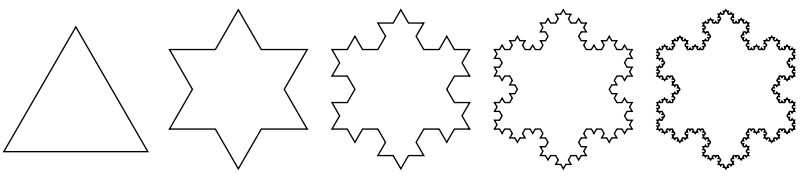
\includegraphics[scale = 0.6]{img/copo-Koch.png}
\caption{Generación del copo de nieve de Koch}
 \label{fig:copo-Koch}
\end{figure}

Esta curva posee la particularidad de tener longitud infinita y a su vez encerrar un área finita. Realmente el copo de Koch no es exactamente un fractal, pues no es totalmente autosimilar, aunque se compone de tres partes idénticas las cuales sí son autosimilares.

\subsection{El triángulo de Sierpinski}

Esta figura, original del polaco Waclaw Sierpinski, es creada de una manera que evoca al conjunto de Cantor, pero en dos dimensiones. Veamos detalladamente el proceso (ver imagen \ref{fig:triangulo-Sierpinski}):

\begin{enumerate}
\item Se parte de un triángulo equilátero de lado 1 (de nuevo la longitud inicial es irrelevante). Uniendo los puntos medios de cada lado obtenemos una partición del triángulo inicial en 4 triángulos equiláteros, del cual extraemos el central. Tenemos por tanto $3=3^1$ triángulos a escala $\frac 1 2 = \left(\frac 1 2\right)^1$ del original.

\item En cada uno de estos tres triángulos equiláteros se repite la operación anterior, obteniendo por tanto $9=3^2$ triángulos, cada uno a escala $\frac 1 4 = \left(\frac 1 2\right)^2$ del original.

\item Repetimos este proceso indefinidamente, de forma que en el paso $n$-ésimo se tienen $3^n$ triángulos, cada uno de ellos a escala $\left(\frac 1 2\right)^n$ del original.
\end{enumerate}

La figura a la que converge este proceso infinito se conoce como triángulo \textbf{S} de Sierpinski.

\begin{figure} [h]
\centering
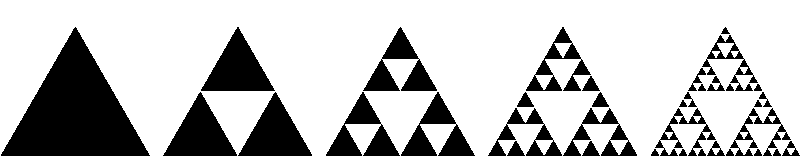
\includegraphics[scale = 0.6]{img/Sierpinski-triangle.png}
\caption{Generación del triángulo de Sierpinski}
 \label{fig:triangulo-Sierpinski}
\end{figure}

\subsection{La alfombra de Sierpinski y la esponja de Menger}

El propio Sierpinski se dio cuenta que con el mismo patrón utilizado para generar \textbf{S} se pueden generar otras formas. Por ejemplo, pensemos que en lugar de partir de un triángulo equilátero partimos de un cuadrado, lo subdividimos en 9 cuadrados de lado $\frac 1 3$ y extraemos el cuadrado central. Repitiendo este proceso indefinidamente con cada uno de los cuadrados que se generan finalmente se obtiene la llamada alfombra de Sierpinski (ver imagen \ref{fig:alfombra-Sierpinski}).

\begin{figure} [h]
\centering
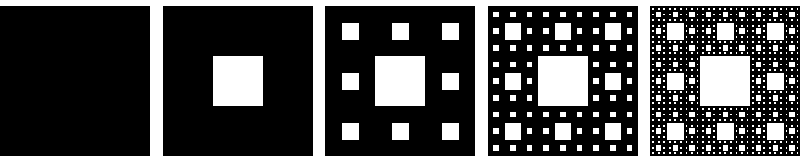
\includegraphics[scale = 0.6]{img/Sierpinski-carpet.png}
\caption{Generación de la alfombra de Sierpinski}
 \label{fig:alfombra-Sierpinski}
\end{figure}

Este proceso también se puede modelar en 3D, obteniendo así la conocida como esponja de Menger o cubo de Magritte, que es una generalización en tres dimensiones de la alfombra de Sierpinski, la cual podemos ver en la imagen \ref{fig:esponja-menger}.

\begin{figure} [h]
\centering
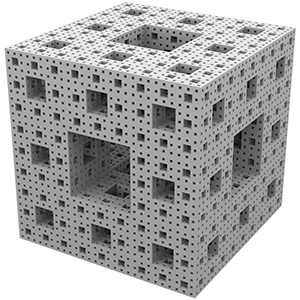
\includegraphics[scale = 0.6]{img/esponja_menger.png}
\caption{Esponja de Menger}
 \label{fig:esponja-menger}
\end{figure}
